\section{Graphentheorie}
\label{sec:graphentheorie}
Da GraphQL es ermöglicht, dass komplexe Beziehungen innerhalb eines Datenmodells in Form von Graphen modelliert werden, benötigen
wir die Graphentheorie, da diese Methoden liefert um Graphen systematisch zu definieren und analysieren.
Desweiteren sind Teile der Testcoverage-Kriterien eng mit Graphenstrukturen verbunden sodass wir gezwungen sind uns
einführend mit der Graphentheorie zu beschäftigen damit wir die Grundlagen erarbeiten, die wir später benötigen werden.
Generell wird es im folgenden eher etwas theoretischer gehalten, die Zusammenhänge werden sich in späteren Kapiteln
erschließen wenn wir Graphen mit GraphQL verbunden oder Tests aus Graphenstrukturen entwickeln.

\subsection{allgemeiner Graph}

Ein Graph ist ein Paar $\textrm{G = (V, E)}$ zweier disjunkter Mengen mit E $\subseteq$ V^2~\cite[vgl. S.2 0.1 Graphen]{graphentheorie}

Elemente von V nennt man Knoten eines Graphens, die Elemente von E nennt man Kanten, Knoten die in einem Tupel von E vorkommen
nennt man auch inzident (benachbart)~\cite[vgl. S.3 0.1 Graphen]{graphentheorie}.
Einen Graphen kann man nun definieren, indem wir zum Beispiel für V = {1, 2, 3} wählen und für E = {(1, 1), (1, 2), (1, 3)}.
Dargestellt werden können Graphen, indem man die Elemente von V als, zum Beispiel, Kreis zeichnet und dann alle Kanten aus E
einzeichnet, indem man die Punkte verbindet~\cite[vgl. S.2 0.1 Graphen]{graphentheorie}.
Eben definierter Graph hat dann folgende Darstellung:

\begin{center}
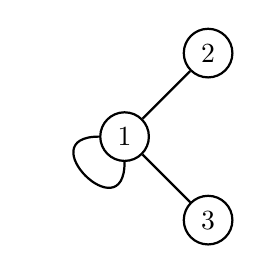
\begin{tikzpicture}[node distance={15mm}, thick, main/.style = {draw, circle}]
    \node[main] (1) {$1$};
    \node[main] (2) [above right of=1] {$2$};
    \node[main] (3) [below right of=1] {$3$};
    \draw (1) to [out=180,in=270,looseness=5] (1);
    \draw (1) -- (2);
    \draw (1) -- (3);
\end{tikzpicture}
\end{center}

Es finden sich auch andere Darstellungsformen für Graphen, hier sei insbesondere die Adjazenzmatrix genannt.
Für unseren Anwendungsfall belassen wir es jedoch bei Punkten und Linien.
Mit dieser Definition lassen sich nun beliebig große, ungerichtete Graphen erstellen.

\subsection{Grundbegriffe der Graphentheorie}

Verschiedene Begriffe sind grundlegend für ein weiterführendes Verständnis der Graphentheorie.
Wir werden hier auf einige dieser Grundbegriffe näher eingehen, insbesondere auf diejenigen die im Testkontext unbedingt benötigt werden.

\subsubsection{Kante}
Die Kante wurde zwar zuvor schon definiert als $e \in E \subseteq V^2$ also ein Tupel $(x, y)$ wobei $x,y \in V$ mit $E$ und $V$ wie in $4.1.1$ definiert.
Hierbei zeigt die Kante, dass die Knoten $x$ und $y$ miteinander verbunden sind.
Äquivalent ist auch die Aussage, dass $y$ und $x$ verbunden sind.
Wir nennen diese Kanten auch ungerichtete Kanten~\cite[vgl. S.3 0.1 Graphen]{graphentheorie}
Wir wollen nun zwei weitere Arten von Kanten definieren.

\subsubsection{gewichtete Kante}

Eine gewichtete Kante fügt einen dritten Parameter zu einer Kante hinzu, sein Gewicht.
Dies ist ein dritter Parameter einer Kante $(x,y)$ wir erweitern also die Definition um einen dritten Parameter
$(x,y,z)$ wobei z meist $z \in \mathbb{R}$ ist.
Solche gewichte können benutzt werden um ideale Wege in Graphen zu finden da sie einer Kante eine Zahl zuweisen, die
als Kosten genutzt werden können.
Gewichtete Kanten werden in unserem Prototypen eine wichtige Rolle spielen allerdings wird bei uns die Kante
keine Zahl aus $\mathbb{R}$ als Gewicht bekommen sondern Objekte aus GraphQL\@.

\subsubsection{gerichtete Kante / gerichteter Graph}

Eine gerichtete Kante besitzt im Gegensatz zu den ungerichteten Kanten eine Orientierung.
Dies bedeutet, dass die Kante $(x,y)$ einen Startknoten und einen Endknoten definieren muss.
Gekennzeichnet wird dies für den Startknoten durch $init()$ und für den Endkonten durch $end()$.
Eine gerichtete Kante vom Knoten $x$ nach $y$ wird somit definiert als $(init(x), end(y))$ \cite[vgl. S.26 Verwandte Begriffsbildungen]{graphentheorie}
Die Einführung von gerichteten Kanten ermöglicht es uns, gerichtete Graphen zu erstellen.
Gerichtete Graphen sind Graphen, die nur gerichtete Kanten besitzen.
Im Prinzip funktionieren gerichtete Kanten wie Einbahnstraßen - es ist nur möglich in die erlaubt Richtung vorzuschreiten.
Die gerichteten Graphen sind besonders wichtig für uns, da alle späteren Analysen von GraphQL auf gerichteten Graphen
basieren.

\subsubsection{Grad eines Knoten}

Der Grad eines Knoten gibt an, wie viele andere Knoten mit diesem Knoten verbunden sind und wird als $d_G(node)$ benannt.
In ungerichteten Graphen ist der Grad eines Knoten $x$ mit 4 Kanten also $d_G(x) = 4$.
Bei gerichteten Graphen unterscheiden wir zwischen Eingangs- und Ausgangsgrad.
Der Eingansgrad ist definiert als Anzahl aller Kanten die auf den Knoten eingehen und der Ausgangsgrad ist genau entgegengesetzt,
die Anzahl aller Kanten die ausgehend vom gewählten Knote sind.

\subsubsection{Pfad / Weg}

Ein Pfad, oft auch Weg genannt, ist eine Sequenz von Knoten die nachfolgend durch Kanten miteinander verbunden sind.~\cite[vgl. S. 7 0.3]{graphentheorie}
Der Pfad von einem Knoten $x$ zu einem Knoten $y$ über Knoten $n_1$ bis $n_7$ hat dann zum Beispiel diese
Struktur $p = \{(x, n2), (n2, n3), (n3, n6), (n6, y)\}$ wobei hierbei gilt,
dass die Kanten $\{(x, n2), (n2, n3), (n3, n6), (n6, y)\} \in E$.
Graphisch würde dies wie folgt aussehen (der Pfad in Rot markiert):

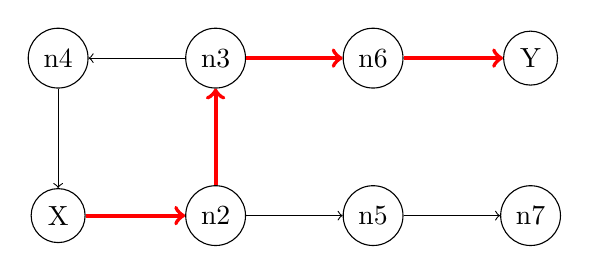
\begin{tikzpicture}
    \node[circle, draw] (n1) at (0,0) {X};
    \node[circle, draw] (n2) at (2,0) {n2};
    \node[circle, draw] (n3) at (2,2) {n3};
    \node[circle, draw] (n4) at (0,2) {n4};
    \node[circle, draw] (n5) at (4,0) {n5};
    \node[circle, draw] (n6) at (4,2) {n6};
    \node[circle, draw] (n7) at (6,0) {n7};
    \node[circle, draw] (n8) at (6,2) {Y};

    \draw[->, red, line width=1.5pt] (n1) -- (n2);
    \draw[->, red, line width=1.5pt] (n2) -- (n3);
    \draw[->] (n3) -- (n4);
    \draw[->] (n4) -- (n1);
    \draw[->] (n2) -- (n5);
    \draw[->, red, line width=1.5pt] (n3) -- (n6);
    \draw[->] (n5) -- (n7);
    \draw[->, red, line width=1.5pt] (n6) -- (n8);
\end{tikzpicture}

Pfade haben immer eine Länge.
Die Länge des Pfades entspricht der Anzahl der Kanten innerhalb dieses Pfades, das bedeutet, dass Pfadl"ange $ = |p|$ wobei $p = \{(x, n2), (n2, n3), (n3, n6), (n6, y)\}$.
Zu beachten ist, dass Pfade in gerichteten Graphen immer die Orientierung der Kanten beachten müssen.
In obigem, gerichteten Pfad wäre also ein Weg $ \{ (X,N4), (N4, N3) \} $ nicht zulässig.

\subsubsection{Zyklus / Kreis}

Ein Zyklus, auch Kreis genannt, ist ein Pfad bei dem gilt, dass der Startpunkt und Endpunkt der Pfadsequenz identisch ist.
Formell bedeutet dies, dass ein Pfad eine Sequenz p = $ \{ (X, e1), (e2, e3), ...., (e_n, X) \}$ ist wobei es auch möglich ist, dass
der Kreis Länge 1 hat also die Sequenz p = $ \{ (X, X) \}$ ist.
Zyklen können in gerichteten und ungerichteten Graphen auftreten wobei das Vorkommen in ungerichtete Graphen eigentlich garantiert ist,
insofern eine Kante existent ist.
Das Auftreten in ungerichteten Graphen ist nicht garantiert aber kann durchaus geschehen.
Der Graph aus vorigem Beispiel definiert exemplarisch den Pfad p = $ \{ (X, n2), (n2, n3), (n3, n4), (n4, X) \}$  welcher ein Kreis ist.
Graphisch hervorgehoben:

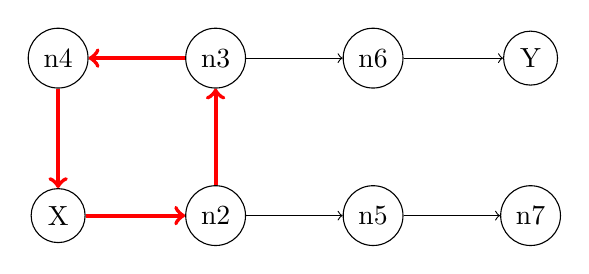
\begin{tikzpicture}
    \node[circle, draw] (n1) at (0,0) {X};
    \node[circle, draw] (n2) at (2,0) {n2};
    \node[circle, draw] (n3) at (2,2) {n3};
    \node[circle, draw] (n4) at (0,2) {n4};
    \node[circle, draw] (n5) at (4,0) {n5};
    \node[circle, draw] (n6) at (4,2) {n6};
    \node[circle, draw] (n7) at (6,0) {n7};
    \node[circle, draw] (n8) at (6,2) {Y};

    \draw[->, red, line width=1.5pt] (n1) -- (n2);
    \draw[->, red, line width=1.5pt] (n2) -- (n3);
    \draw[->, red, line width=1.5pt] (n3) -- (n4);
    \draw[->, red, line width=1.5pt] (n4) -- (n1);
    \draw[->] (n2) -- (n5);
    \draw[->] (n3) -- (n6);
    \draw[->] (n5) -- (n7);
    \draw[->] (n6) -- (n8);
\end{tikzpicture}

\subsection{Zusammenfassung}

Wir haben nun eine kleine mathematische Einführung in das Gebiet der Graphentheorie hinter uns.
Mithilfe der hier erarbeiteten Begriffe und Definitionen werden wir im folgenden verehrt arbeiten.
Insbesondere wenn wir die Coverage-Algorithmen im Bezug des Testens einführen benötigen wir das hier erarbeitete Wissen.





